\documentclass[12pt]{article}
\usepackage{graphicx} 
\usepackage{float}
\usepackage{placeins}
\usepackage{amsmath}
\usepackage{hyperref}

\author{Vale Fernando Alexis}
\begin{document}
\section{Introducción}
La ionosfera existe entre aproximadamente entre los 50 y 1000 km sobre la 
superficie de la tierra. La radiación del sol ioniza átomos y moléculas en 
esta región, liberando electrones y creando una región de iones y electrones 
libres. Sometidos al campo eléctrico externo de una señal de radio, estos 
electrones libres y iones experimentan una fuerza que les ocasionará un 
movimiento. Sin embargo, dado que la masa de los iones es mucho mayor a la masa 
de los electrones, los movimientos iónicos son relativamente pequeños, lo mismo 
ocurre con la colisión de electrones.
La ionización de los rayos del sol produce densidades de electrones libres del 
orden de $10^{10} $ a $10^{12}$ electrones por metro cúbico. Las capas de alta densidad 
de electrones reciben nombres especiales: son llamadas capas D, E, F.
Durante el día, la capa F se divide en dos capas llamadas F1 y F2, mientras que 
la capa D desaparece completamente por la noche. 
Las ondas de radio por debajo de los 40 MHz se ven afectadas significativamente 
por la ionosfera, principalmente porque las ondas de radio en este rango de 
frecuencia se reflejan de manera efectiva.

    \begin{figure}[ht]
    \centering
    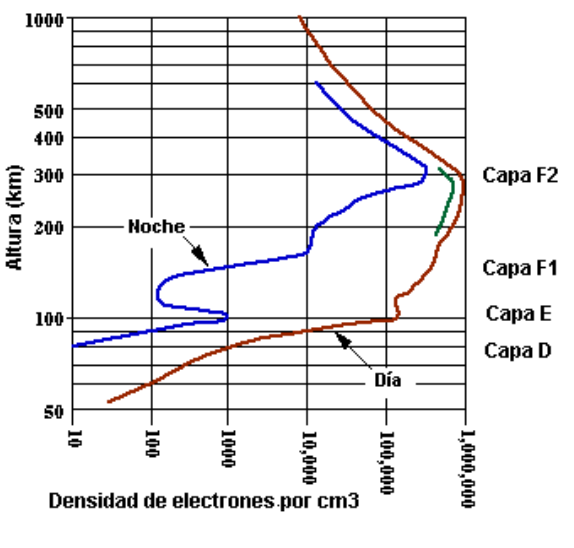
\includegraphics[width=0.5\textwidth]{./Imagenes/DensidadElectrones.png}
    \caption{Densidad de Electrones vs Altura}
    \label{fig:first}
    \end{figure}
    \FloatBarrier
\subsection{Propagación}
Las ondas de radio de alta frecuencia (HF) se utilizan en varias aplicaciones, como comunicaciones 
de larga distancia, detección y seguimiento por radar, utilizando la ionosfera como reflector para
 aumentar el alcance en tierra. Debido a la complejidad teórica de la propagación de ondas 
 electromagnéticas a través de la ionosfera, que es un plasma magnetizado, todavía sigue siendo 
 un desafío establecer enlaces de radio y posiciones exactas con los sistemas de radar. El \textbf{ray tracing} 
 se utiliza habitualmente para solucionar este problema por que permite calcular la trayectoria exacta 
 de las ondas de radio, aunque requiere un conocimiento preciso de la ionosfera, que es un medio muy 
 variable. A sus variaciones regulares (por ejemplo, diarias y estacionales), se suman las perturbaciones 
 transitorias, como las perturbaciones ionosféricas viajeras(TID - Traveling Ionospheric Disturbances).
 Observando el efecto de los TID de mediana escala (MSTID) sobre algunas características de las trayectorias 
 de los rayos HF. Las MSTID a menudo se asocian con la acción de ondas de gravedad atmosféricas (GW), 
 con períodos que van desde varios minutos hasta menos de una hora y velocidades de ~50 a 300 m/s.
 El efecto de los TID en las trayectorias de los rayos puede provocar un desplazamiento Doppler de 
 la señal recibida y cambios en las trayectorias de los rayos, lo que a su vez puede producir fluctuaciones 
 aparentes en los ecos de retorno del objetivo en aplicaciones de radar y provocar errores de registro de 
 coordenadas en radares sobre el horizonte. \par
 También puede limitar el rendimiento de los algoritmos de detección de objetivos debido al rango asociado y 
 la desviación azimut que puede hacer que un objetivo fijo parezca moverse varias decenas de kilómetros en unos 
 pocos minutos.
 
\section{La Ionosfera y sus diferentes capas}
La ionosfera es una región de la atmósfera terrestre que está ionizada por la radiación 
solar y se extiende aproximadamente desde los 50 Km hasta los 1000 Km de altitud. Se 
puede dividir en varias capas o regiones, cada una con características específicas:\par
\begin{itemize}
    \item Capa D:
    \begin{itemize}
        \item \textbf{Altitud}: Aproximadamente entre 50 Km y 90 Km.
        \item \textbf{Características}: Es la capa más baja y menos ionizada. Pre\-do\-mi\-na
        durante el día y práctimanente desaparece durante la noche. La ionización es causada
        principalmente por la radiación solar de baja energía y la radiación cósmica.
    \end{itemize}
    \item Capa E:
    \begin{itemize}
        \item \textbf{Altitud}: Aproximadamente entre 90 Km y 150 Km.
        \item \textbf{Características}: También conocida como la región Kennelly-Heaviside, 
        esta capa es más ionizada que la capa D. La ionización se debe a la radiacion ultravioleta
        y los rayos X del sol. \par
        Se mantiene durante el día y disminuye significativamnte durante la noche.
    \end{itemize}
    \item Capa F:
    \begin{itemize}
        \item \textbf{Altitud}: Aproximadamente entre 150 Km y 1000 Km.
        \item \textbf{Características}: Esta capa se divide en dos subcapas durante el día:
            \begin{itemize}
                \item \textbf{F1}: Aproximadamente entre 150 Km y 250 Km. Se forma durante el día 
                y desaparece durante la noche.
                \item \textbf{F2}: Aproximadamente entre 250 Km y 1000 Km. Es la capa más alta y más persistente,
                manteniéndose tanto de día como de noche. La ionización en esta capa es más 
                fuerte debido a la radiación ultravioleta extrema y los rayos X.
            \end{itemize}
    \end{itemize}
\end{itemize}
La capa \textbf{F2} es la más importante para la reflexión de las ondas de radio en la banda de alta 
frecuencia (HF), permitiendo la comunicación a larga distancia y el funcionamiento de los radares
transhorizontales (OTHR)


\subsection{Frecuencias para el aprovechamiento de la Ionosfera}
El rango de frecuencias utilizado para aprovechar la ionosfera como reflector 
en aplicaciones de radar, específicamente en los radares  transhorizontales (OTHR),
es tipicamente dentro de las frecuencias de ondas decamétricas. Este rango se
encuentra entre los \textbf{3 MHz y 30 Mhz} en la banda de frecuecias de alta 
frecuencia (HF). Dentro de este rango:
\begin{itemize}
    \item \textbf{Frecuencias bajas(3-10 MHz)}: Son usadas para alcanzar distancias
    más largas debido a su mejor propagación a través de la ionosfera durante la noche 
    en condiciones de baja actividad solar.
    \item  \textbf{Frecuencias altas(10-30 MHz)}: Se utilizan para distancias más
    cortas y son más efectivas durante el día o en condiciones de alta actividad solar.
\end{itemize}
Estos rangos de frecuencia permiten que las ondas de radio sean reflejadas por la 
ionosfera, lo que permite a los radares detectar objetos más allá del horizonte terrestre,
significativamente el rango de detección.

\subsection{Alcances de los Radares transhorizontales(OTHR)}
Los alcances en distancia de los radares transhorizontales varían según la frecuencia 
utilizada y las condiciones ionosféricas. Por ejemplo:
\begin{itemize}
    \item Frecuencias bajas (3-10 MHz):
    \begin{itemize}
        \item \textbf{Alcance típico}: Entre 1000 Km y 4000 Km.
        \item \textbf{Condiciones óptimas}: Durante la noche o en periodos de baja actividad
        solar, cuando la ionosfera es más estable y densa a altitudes más bajas.
    \end{itemize}
    \item Frecuencias altas(10-30 MHz):
    \begin{itemize}
        \item \textbf{Alcance típico}: Entre 500 Km y 2000 Km.
        \item \textbf{Condiciones óptimas}: Durante el día o en periodos de alta actividad
        solar, cuando la ionosfera es más ionizada y densa a moayores altitudes.
    \end{itemize}
\end{itemize}
\subsection{Factores que afectan el alcance}
\begin{itemize}
    \item \textbf{Hora del día}: La ionosfera cambia considerablemente entre el día y 
    la noche.Durante el día, la ionosfera es más ionizada debido a la radiación solar, 
    lo que afecta la reflexión de ondas de radio.
    \item \textbf{Actividad solar}: Altos niveles de actividad solar puedeen aumenar la
    ionización de la ionosfera, afectando la capacidad de las ondas de radio ara ser reflejadas.
    \item \textbf{Condiciones atmosféricas}: Las variaciones en la densidad de la ionosfera 
    debido a las condiciones atmosféricas tambien influyen en el alcance del radar.
\end{itemize}

\subsection{Efectos de la Actividad Solar}
La actividad solar afecta la reflexión de las ondas de radio en la ionosfera debido a 
su influencia en la ionización de esta región de la atmósfera. La ionización de la 
ionosfera depende principalmente de la radiación solar, particularmente de los rayos 
ultravioleta (UV) y los rayos X.
\begin{itemize}
    \item Alta Actividad Solar:
        \begin{itemize}
            \item \textbf{Características}: Durante periodos de alta actividad solar, como 
            los máximos solares en el ciclo solar de 11 años, la radiación UV y los rayos 
            X aumentan, incrementando la ionización en todas las capas de la ionosfera.
            \item \textbf{Impacto en la Reflexión}: La mayor ionización puede hacer que las 
            capas más altas de la ionosfera, como la capa F2, sean más densas y reflectivas 
            para las ondas de radio de alta frecuencia (HF). Sin embargo, la excesiva ionización 
            también puede provocar una mayor absorción de las ondas en las capas más bajas, 
            como la capa D, especialmente durante el día.
            \item \textbf{Condiciones Óptimas}: Frecuencias más altas(10-30 MHz) tien\-den a reflejarse 
            mejor durante estos periodos, permitiendo alcances más largos.
            \item \textbf{Condiciones Subóptimas}: En casos de actividad solar estrema\-damente
            alta, como durante las tormentas solares, la ionosfera puede volveerse demasiado turbulenta, 
            causando irregularidades y pérdida de la señal reflejada.
        \end{itemize}
    \item Baja Actividad Solar:
        \begin{itemize}
            \item \textbf{Características}: Durante periodos de baja actividad solar, como los 
            mínimos solares, la radiación UV y los rayos X disminuyen, resultando en una menor 
            ionización de la ionosfera.
            \item \textbf{Impacto en la Reflexión}: La ionización reducida puede limitar la 
            efectividad de la reflexión de las ondas de radio, especialmente para las frecuencias 
            más altas. Las frecuencias más bajas (3-10 MHz) pueden reflejarse mejor en estas 
            condiciones.
            \item \textbf{Condiciones Óptimas}: Frecuencias más bajas tienden a reflejarse mejor, 
            permitiendo comunicaciones y detección a largas distancias durante la noche.
            \item \textbf{Condiciones Subóptimas}: Durante el día, la reflexión puede ser menos 
            efectiva debido a la menor ionización.
        \end{itemize}
\end{itemize}

\subsection{ Mejores y Peores Condiciones}
\begin{itemize}
  \item Mejores Condiciones(Óptimas):
    \begin{itemize}
      \item \textbf{Moderada a Alta Actividad Solar}: Permite una buena io\-ni\-zación de la capa F2, 
      facilitando la reflexión de las ondas de radio de alta frecuencia, especialmente durante el 
      día.
      \item \textbf{Noche de Baja Actividad Solar}: Las frecuencias más bajas pueden reflejarse
      mejor, permitiendo comunicaciones a larga distancia.
  \end{itemize}
\end{itemize}
\begin{itemize}
  \item Peores Condiciones:
  \begin{itemize}
    \item \textbf{Tormentas solares}: Pueden causar una excesiva turbulencia en la ionosfera, 
    resultando en pérdida de señal y comunicaciones i\-nes\-ta\-bles.
    \item \textbf{Actividad Solar Extremadamente Baja}: Puede resultar en una ionización 
    insuficiente, dificultando la reflexion de las ondas de radio, especialmente durante el día.
  \end{itemize} 
\end{itemize}
Resumiendo, las condiciones óptimas para la reflexión de las ondas de radio en la ionosfera 
ocurren durante periodos de moderada a alta actividad solar, donde la ionización es suficiente para
reflejar las ondas, pero no tan intensa como para causar turbulencia o absorción excesiva


\section{Introdución a la interpolación}
  
La interpolación es una técnica utilizada para estimar valores intermedios 
entre puntos de datos conocidos. A continuación, se describen varios métodos 
de interpolación, cada uno con sus características y aplicaciones:
\subsection{Tipos}
\subsubsection{Interpolación Lineal (\texttt{linear})}
Este es el método más simple, que conecta dos puntos adyacentes con una 
línea recta. Es adecuado para datos que siguen una tendencia lineal y 
proporciona una transición suave entre puntos.

\subsubsection{Interpolación Más Cercana (\texttt{nearest})}
Este método asigna al punto interpolado el valor del punto de datos más
 cercano. Es útil cuando se requiere que los valores interpolados sean 
 iguales a los puntos de datos originales, sin generar valores intermedios.

\subsubsection{Interpolación Más Cercana hacia Arriba (\texttt{nearest-up})}
Similar a \texttt{nearest}, pero siempre selecciona el siguiente valor más 
cercano hacia arriba. Es útil cuando se desea evitar subestimaciones.

\subsubsection{Interpolación por Zonas (\texttt{zero})}
Este método mantiene constantes los valores de la interpolación hasta el 
siguiente punto de datos, lo que produce una función por partes. Es útil 
en sistemas donde los valores cambian bruscamente.

\subsubsection{Interpolación Lineal Segmentada (\texttt{slinear})}
Una versión mejorada de la interpolación lineal, que utiliza segmentos 
lineales entre puntos de datos. Es más suave que la interpolación lineal 
simple, especialmente en datos no lineales.

\subsubsection{Interpolación Cuadrática (\texttt{quadratic})}
Utiliza polinomios de segundo grado para interpolar entre puntos. 
Es más preciso que los métodos lineales en datos con curvaturas suaves y no lineales.

\subsubsection{Interpolación Cúbica (\texttt{cubic})}
Este método utiliza polinomios de tercer grado y es altamente adecuado 
para datos que requieren una curva suave y continua. Proporciona una mejor 
aproximación que los métodos lineales y cuadráticos.

\subsubsection{Interpolación Previa (\texttt{previous})}
Asigna al punto interpolado el valor del punto de datos anterior. Es útil en 
situaciones donde los valores deben permanecer constantes hasta el próximo 
cambio de datos.

\subsection{Comparación de Métodos}
Cada método de interpolación tiene aplicaciones específicas dependiendo de la 
naturaleza del conjunto de datos y la suavidad deseada en la curva de interpolación. 
Los métodos lineales son simples y rápidos, pero pueden ser inexactos en datos 
con cambios no lineales. Los métodos cuadráticos y cúbicos son más complejos, 
pero ofrecen una mayor precisión y suavidad en la interpolación.
\section{Interpolación Spline Cuadrática}
  Es una técnica para crear una función suave que pase a través de un conjunto 
  de puntos dados. Muy diferente a la interpolación lineal, que conecta los puntos 
  con segmentos de línea recta. En éste caso se usa polinomios (grado 2) para crear
  dicha curva \textbf{suave}.\par
    \subsection{Concepto Básico}
    La idea es dividir el rango de datos en segmentos y, para cada segmento, ajustar 
    un polinomio cuadrático (de segundo grado). Estos polinomios están construidos de 
    manera que sean continuos en el punto de unión, es decir, la curva es suave en todos 
    los puntos de datos.
    \subsection{Pasos para Implementar la Interpolación Spline Cuadrática}
     \begin{enumerate}
        \item Dividir los puntos de datos en segmentos. Si tienes $n$ puntos, tendrás $n-1$ segmentos.
        \item Ajustar un polinomio cuadrático a cada segmento. La forma general de un polinomio cuadrático es:
        \[S_i(x) = a_i (x - x_i)^2 + b_i (x - x_i) + c_i\]
        donde $a_i$, $b_i$, y $c_i$ son los coeficientes del polinomio para el segmento $i$, y $x_i$ es el punto 
        de inicio del segmento.
        \item Imponer condiciones de continuidad: Los polinomios deben coincidir en el valor y en la primera 
        derivada en los puntos de unión.
      \end{enumerate}
\section{Interpolación Spline Cúbica}
  La interpolación Spline Cúbica: Es una Técnica matemática utilizada para 
aproximar una curva SUAVE que pasa por un conjunto dado de puntos. Es especialmente
útil en situaciones en las que tenemos puntos de datos dispersos y queremos crear 
una curva continua que captura una tendencia general.
Luego podemos usar esa curva apara encontrar información valiosa sobre nuestros
datos. 

\section{Función splprep - SciPy}
  La función \textbf{splprep} es parte del módulo \texttt{scipy.interpolate} en 
Python y se utiliza para generar una interpolación paramétrica en el espacio 
multidimensional utilizando splines. Esta función es especialmente útil cuando 
tienes datos dispersos en varias dimensiones y deseas suavizar una curva o una 
superficie que pasa a través de esos puntos de control.

\section*{¿Cómo funciona \texttt{splprep}?}
\texttt{scipy.interpolate.splprep} toma como entrada un conjunto de datos que 
representan puntos en el espacio, y devuelve un spline paramétrico que pasa cerca 
de esos puntos. Un \textbf{spline} es una función matemática compuesta por 
segmentos de polinomios que se ajustan suavemente en los puntos de control.

\section*{Parámetros importantes}

\begin{itemize}
    \item \texttt{[x, y, z, \ldots]}: Una lista de \texttt{arrays} que contienen 
    las coordenadas de los puntos en el espacio. Si tienes una curva 2D, proporcionas 
    \texttt{[x, y]}, para una superficie 3D, proporcionas \texttt{[x, y, z]}.
    \item \texttt{s}: Factor de suavizado. Un valor más pequeño hará que el spline 
    pase más cerca de los puntos de datos originales. Un valor más grande permitirá 
    más suavizado. Si \texttt{s=0}, el spline pasará \textbf{exactamente} por los 
    puntos de datos.
    \item \texttt{k}: El grado del spline. Por defecto es \texttt{k=3}, lo que 
    significa que se utiliza un spline cúbico. Puedes cambiarlo a \texttt{k=2} para 
    un spline cuadrático, por ejemplo.
    \item \texttt{u}: Si deseas controlar el parámetro que corresponde a cada punto, 
    puedes proporcionarlo. De lo contrario, se genera automáticamente en el rango 
    \texttt{[0, 1]}.
\end{itemize}

\section*{Resultados}

\begin{itemize}
    \item \texttt{tck}: Es una tupla que contiene tres elementos: el vector de nodos, 
    los coeficientes del spline, y el grado del spline.
    \item \texttt{u}: El valor de los parámetros para los puntos de datos originales.
\end{itemize}
\section{Función splev - SciPy}
  La función \textbf{splev} es parte del módulo \texttt{scipy.interpolate} y se 
utiliza para evaluar un spline en puntos específicos. Después de haber ajustado 
un spline usando \texttt{splprep}, puedes usar \texttt{splev} para calcular el 
valor del spline en cualquier conjunto de parámetros.

\subsection*{¿Cómo funciona \texttt{splev}?}

\textbf{splev} toma un conjunto de valores de parámetros y un objeto spline 
(generalmente el resultado de \texttt{splprep}) y devuelve los valores 
correspondientes del spline en esos puntos.

\subsection*{Parámetros importantes}

\begin{itemize}
    \item \texttt{u}: Un array de valores de parámetros en los cuales deseas 
    evaluar el spline. Estos valores deben estar en el rango \texttt{[0, 1]} 
    si no has especificado otro rango en \texttt{splprep}.
    \item \texttt{tck}: El objeto spline, que es el resultado de la función 
    \texttt{splprep}. Contiene la información sobre el spline, incluyendo el 
    vector de nodos, los coeficientes y el grado del spline.
\end{itemize}

\subsection*{Resultado}

\begin{itemize}
    \item \texttt{values}: Un array de valores que corresponde a la evaluación 
    del spline en los puntos especificados por \texttt{u}. Si estás trabajando 
    en un espacio multidimensional, este será una lista de arrays, uno para cada 
    dimensión.
\end{itemize}



\section{Redes Neuronales}
  \begin{figure}[ht]
    \centering
    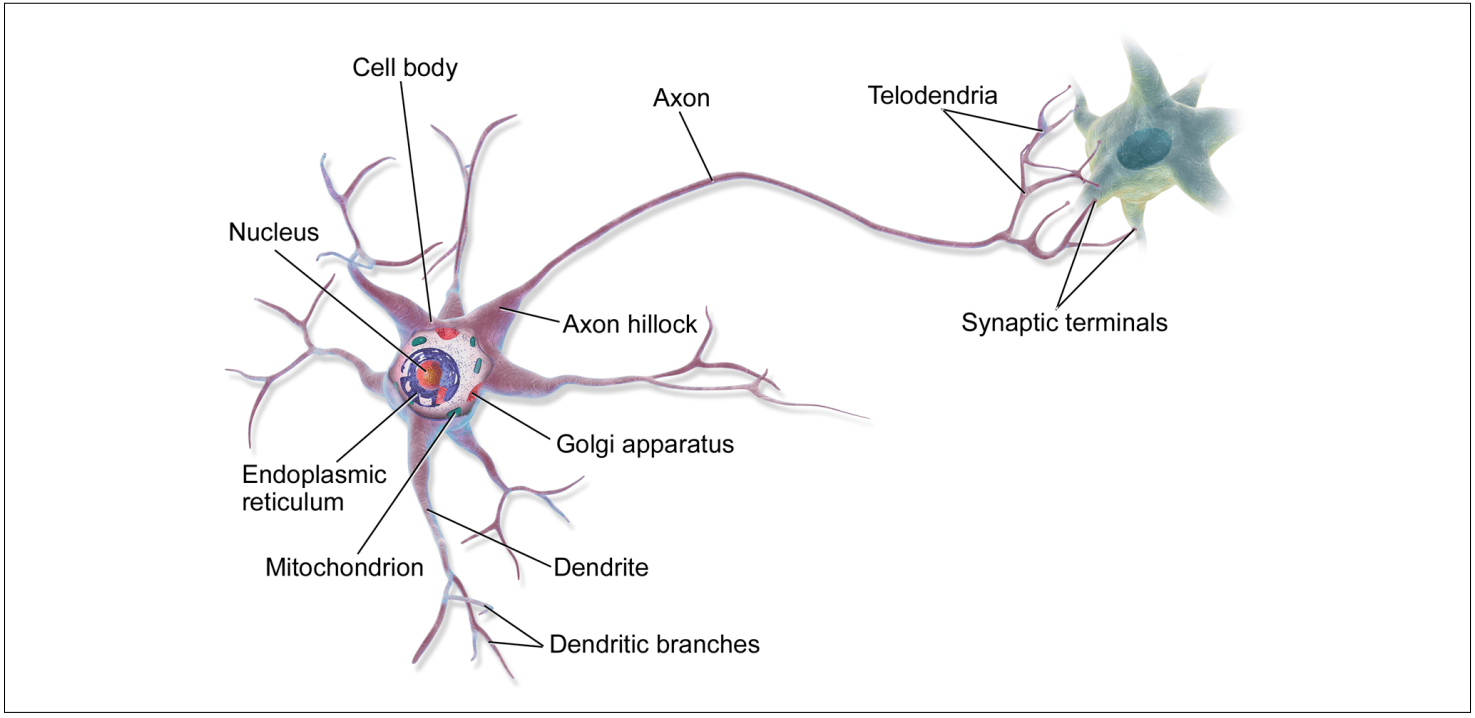
\includegraphics[width=0.8\textwidth]{./Imagenes/NeuronaBiologica.png}
    \caption{Neoruona Biológica}
    \label{fig:segunda}
  \end{figure}
  
  \subsection{Red Neuronal y Red Neuronal Artificial}
  Una \textbf{Red Neuronal} es un sistema de procesamiento de información inspirado en la estructura y 
  funcionamiento del cerebro humano. Está compuesta por un conjunto de unidades llamadas neuronas, 
  que están interconectadas entre sí. Cada neurona recibe una entrada, la procesa y transmite una 
  salida, similar al comportamiento de las neuronas biológicas.\par
  \medskip \noindent
  Una \textbf{Red Neuronal Artificial (RNA)} es un modelo computacional diseñado para simular el funcionamiento 
  de las redes neuronales biológicas. Estas redes están formadas por capas de neuronas artificiales o nodos. 
  Las RNA se utilizan para realizar tareas de reconocimiento de patrones, clasificación, regresión y otras aplicaciones 
  de inteligencia artificial.\par
  \medskip
  \textbf{Diferencias clave:}
  \begin{itemize}
    \item \textbf{Red Neuronal (biológica):} Se refiere a la red de neuronas en el cerebro u otros sistemas nerviosos, responsables de 
    procesar la información en organismos vivos.
    \item \textbf{Red Neuronal Artificial:} Es un modelo matemático y computacional que emula el comportamiento de las redes 
    neuronales biológicas, utilizado en el ámbito de la inteligencia artificial y el aprendizaje automático.
  \end{itemize}
  \subsection{El Perceptrón}
  El \textbf{Perceptrón}   es una de las arquitecturas ANN más simples, inventada en 1957 por Frank Rosenblatt. 
  Es un modelo matemático inspirado en el funcionamiento de las neoronas biológicas.
  
  \textbf{Componentes del Perceptrón}

  \begin{itemize}
      \item \textbf{Entradas:}
      \begin{itemize}
          \item El perceptrón recibe múltiples entradas, cada una asociada con un peso. Estas entradas pueden ser características de un conjunto de datos.
      \end{itemize}
      
      \item \textbf{Pesos:}
      \begin{itemize}
          \item A cada entrada se le asigna un peso que representa la importancia de esa entrada. Los pesos se ajustan durante el proceso de entrenamiento.
      \end{itemize}
      
      \item \textbf{Suma ponderada:}
      \begin{itemize}
          \item El perceptrón calcula una suma ponderada de las entradas, es decir, cada entrada se multiplica por su peso correspondiente y luego se suman.
          \[
          z = \sum_{i=1}^{n} w_i \cdot x_i + b
          \]
          Donde \( z \) es la suma ponderada, \( w_i \) son los pesos, \( x_i \) son las entradas, y \( b \) es el sesgo (bias).
      \end{itemize}
    
    \item \textbf{Función de activación:}
    \begin{itemize}
        \item El perceptrón utiliza una función de activación para determinar la salida. La función de activación más 
        simple es la función escalón, que devuelve 1 si la suma ponderada es mayor que un umbral, y 0 en caso contrario.
        \[
        y = 
        \begin{cases} 
        1 & \text{si } z > \text{umbral} \\
        0 & \text{si } z \leq \text{umbral}
        \end{cases}
        \]
    \end{itemize}
    
    \item \textbf{Salida:}
    \begin{itemize}
        \item La salida del perceptrón es un valor binario (0 o 1), lo que lo convierte en un clasificador lineal.
    \end{itemize}
\end{itemize}
  \section{Funciones de Activación}
    \href{https://www.datacamp.com/es/tutorial/introduction-to-activation-functions-in-neural-networks}{Funciones de activación}
    
    Las funciones de activación son una componenete integral de las \textbf{redes neoronales} que les permite aprender
    patrones complejos en los datos. Transforman la señal de entrada de un nodo de una red 
    neuronal en una señal de salida que pasa a la capa siguiente. \par
    \begin{figure}[H]
      \centering
      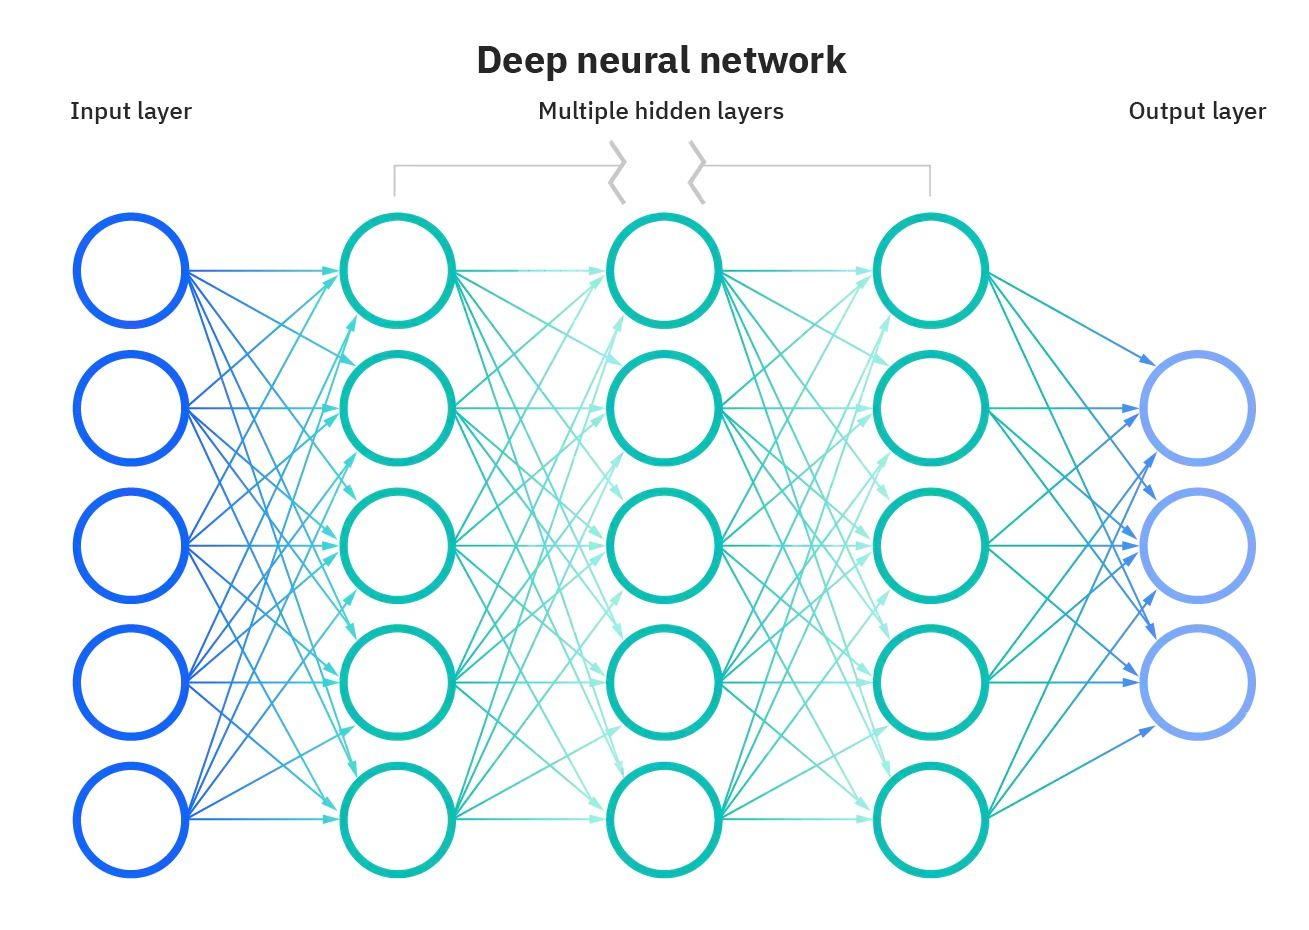
\includegraphics[width=0.8\textwidth]{./Imagenes/FuncionesdeActivacion.png}
      \caption{Representacion de Red Neuronal}
      \label{fig:tercera}
    \end{figure}
    
    \noindent
    Sin funciones de activación, las redes neuronales solo consistirían en ope\-ra\-ciones lineales como la multiplicación de matrices. 
    Todas las capas realizarían transformaciones lineales de la entrada, y no se introducirían no linealidades.
    \subsection*{Tipos de funciones de Activación}
    Cada función de activación tiene sus propias propiedades y es adecuada para determinados casos de uso.
    Utilizar la función de activación adecuada para la tarea conduce a un entrenamiento más rápido y 
    a un mejor rendimiento.
    \subsection*{Función de Activación Lineal}
    \begin{figure}[H]
      \centering
      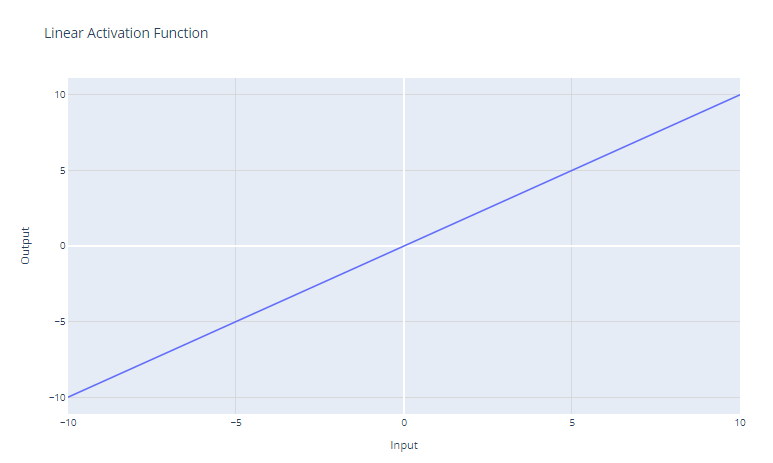
\includegraphics[width=0.8\textwidth]{./Imagenes/funcionActivacionLineal.png}
      \caption{Representacion de Red Neuronal}
      \label{fig:cuarta}
    \end{figure}
    
    La función de activación lineal es la función de activación más sencilla, definida como:
    \[ f(x) = x \]
    El principal caso de uso de la función de activación lineal es en la capa de salida de una red neuronal 
    utilizada para la regresión. Para los problemas de regresión en los que queremos prever un valor numérico, 
    utilizar una función de activación lineal en la capa de salida garantiza que la red neuronal produzca un 
    valor numérico. La función de activación lineal no reduce ni transforma la salida, por lo que se devuelve 
    el valor real previsto.\par
    Sin embargo, la función de activación lineal rara vez se utiliza en las capas ocultas de las redes neuronales. 
    Esto se debe a que no proporciona ninguna no linealidad.

    \subsection*{Función de Activación Sigmoide}
      \begin{figure}[H]
        \centering
        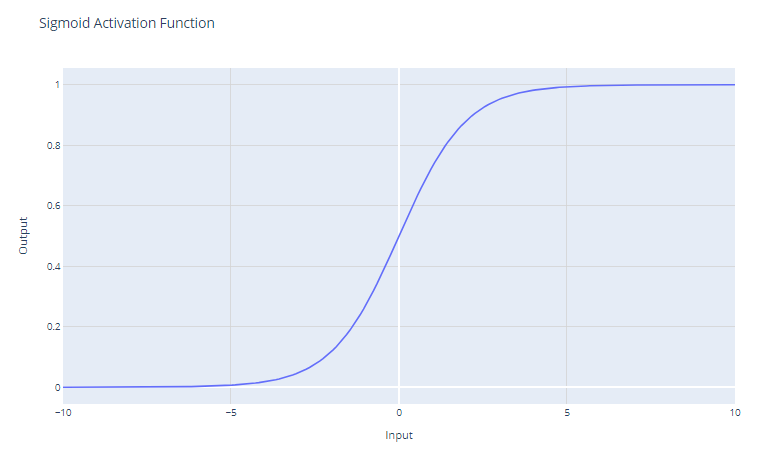
\includegraphics[width=0.8\textwidth]{./Imagenes/funcionSigmoide.png}
        \caption{Función de Activación Sigmoide}
        \label{fig:quinta}
      \end{figure}
    
      La función de activación sigmoide, a menudo representada como \(\sigma(x)\), es una función infinitamente diferenciable 
      históricamente importante en el desarrollo de las redes neuronales
      \[ f(x) = \frac{1}{1+e^{-x}}\]
      Toma una entrada de valor real y la reduce a un valor entre 0 y 1. La función sigmoide tiene una curva en forma de ``S'' 
      que tiende a 0 para los números negativos grandes y a 1 para los números positivos grandes. Los resultados pueden interpretarse 
      fácilmente como probabilidades, lo que la hace natural para los problemas de clasificación binaria.
    \end{document}
